\chapter{General Purpose computing on Graphical Processing Units}
\label{sec:gpgpu}

The original intended use for GPUs was graphics processing, hence its name.
Recently, GPUs have been increasingly used for other purposes - a trend commonly known as General Purpose processing in Graphics Processing Units (GPGPU).
%Using GPU for other applications other than graphic processing, commonly known as GPGPU, has become a trend in recent years.
GPU present a solution for "extreme-scale, cost-effective, and power-efficient high performance computing" \cite{Chen2012}.
Furthermore, GPUs are common in consumer desktops and laptops, effectively bringing this computation power to the masses.

GPUs were typically useful for users that required high performance graphics computation.
Other applications were soon explored as users from different fields realized the high parallel computation power of these devices.
However, the architecture of the GPUs themselves has been strictly oriented toward the graphics computing until the appearance of specialized GPU models designed for data computation (e.g. NVIDIA Tesla).

GPGPU application on several fields and algorithms has been reported with significant performance increase, e.g. application on the K-Means algorithm \cite{Bai2009,Wu2011,Zechner2009,Wu2009a}, hierarchical clustering \cite{Shalom2009,ArulShalom2011}, document clustering \cite{gao20xx}, image segmentation \cite{Sirotkovi2012}, integration in Hadoop clusters \cite{Malakar2013,Grossman2013}, among other applications.

%TODO add refs for energy
Current GPUs pack hundreds of cores and have a better energy/area ratio than traditional infrastructure.
GPU work under the SIMD framework, i.e. all the cores in the device execute the same code at the same time and only the data changes over time.

\section{Programming GPUs}

% old part, i.e. shading models, DirectX, OpenGL, grahics pipeline
In the very beginning of GPGPU, programming was done directly through graphics APIs.
Programming for GPUs was traditionally done within the paradigm of graphics processing, such as DirectX and OpenGL.
If researchers and programmers wanted to tap into the computing power of a GPU they had to learn and use these APIs and frameworks, which is a challenging task since their general problems had to be modelled to the graphics-oriented primitives \cite{Misi2012}.
With the appearance of DirectX 9, shader programming languages of higher level became available (e.g. C for graphics, DirectX High Level Shader Language, OpenGL Shading Language), but they were still inherently graphics programming languages, where computation must be expressed in graphics terms. 

% new part, i.e. interest in GPGPU sparkled unified devices and frameworks
% overview of recent programming models, CUDA is computing framework, OpenCL is a standard
More recent programming models, such as CUDA and OpenCL, removed a lot of that burden by exposing the power of GPUs in a way closer to traditional programming.
Currently, the major programming models used for computation in GPU are OpenCL and CUDA.
While the first is widely available in most devices, the latter is only available for NVIDIA devices.

% give references for GPU MapReduce
As Google's MapReduce computing model has increasingly become a standard for scalable and distributed computing over big data, attempts have been made to port the model to the GPU \cite{Ji2011,Xin2012,He2008}.
This translates in using the same programming model over a wide array of computing platforms.


\section{OpenCL vs CUDA}
% TODO rewrite this on terms of a better comparisson NEEDS REFS

Presently, the most mature programming models are CUDA and OpenCL.
CUDA appeared first and is supported only by NVidia devices.
It is also the most mature of the two and performs well since it was designed alongside with the hardware architecture of the supporting devices.
OpenCL has the advantage of portability, but that comes with issues of performance portability.
Both models are, in fact, very similar and literature suggests that porting the code from one to the other requires minimal changes \cite{Karimi2010,Su2012}.
Literature also reports that CUDA performs better than OpenCL \cite{Su2012} for equivalent code.

% TODO CUDA and OpenCL comparison; they are very similar in lots of ways; languanges they support (Python, Java, C, Pascal,...)


% TODO performance portability problem, how the performance problem can be mitigated and even eliminated by careful choice of compiler parameters, device aware application and so on (Fang2011)


% TODO This should go for methodology
% In the end, the choice of GPU computing framework was CUDA.
% All the infrastructure available for developing and testing supports CUDA.
% Another reason for the choice is that all the work is being developed in Python and Python has a CUDA API of very high level - part of the Numba module developed by Continuum Analytics. 


\section{Overview of CUDA}

%TODO needs refs, it is mostly the C CUDA programming guide

This section presents an overview of the CUDA programming model and its main concepts and characteristics.
For a more thorough and extensive explanation of this topic, the CUDA C Programming Guides \cite{Nvidia2014}, the source of the present review, should be consulted.
A GPU is comprised by one or several streaming processors (or multiprocessor).
Each of these processors contains several simpler processors, each of which execute the same instruction at the same time at any given time.
In the CUDA programming model, the basic unit of computation is a \emph{thread}.
Threads are grouped into \emph{blocks} which are part of the block \emph{grid}.
The number of threads in a block is typically higher than the number of processors in a multiprocessor.
For that reason, the hardware automatically divides the threads from a block into smaller batches, called \emph{warps}.
This hierarchy is represented in Figure \ref{fig:gridthread}.
The computation of one block is independent from other blocks and each block is scheduled to one multiprocessor, which means that more multiprocessors results in more blocks being processed at the same time, as represented in Figure \ref{fig:blockprocessor}.

\begin{figure}[ht]
\centering
\begin{minipage}[b]{.45\textwidth}
	\centering
	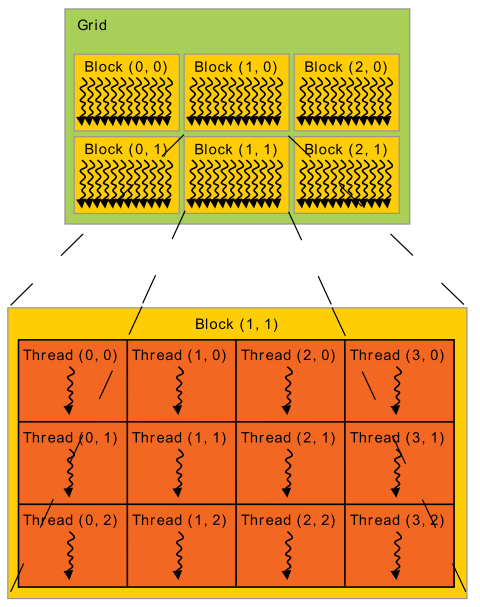
\includegraphics[width=.95\textwidth]{stateofart/gpgpu/threadgrid}
	\captionof{figure}{Thread hierarchy \cite{Nvidia2014}.}
	\label{fig:gridthread}  
\end{minipage}
\begin{minipage}[b]{.45\textwidth}
    \centering
    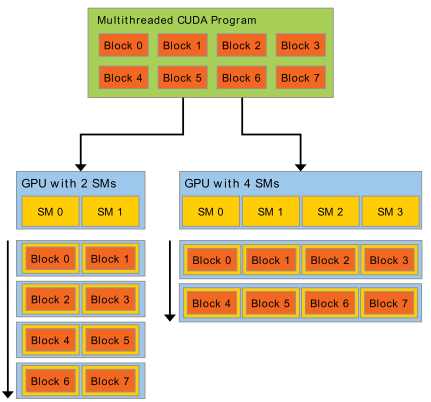
\includegraphics[width=.95\textwidth]{stateofart/gpgpu/blockprocessor}
    \captionof{figure}{Distribution of thread blocks is automatically scaled with the increase of the number of multiprocessors \cite{Nvidia2014}.}%Automatic scalability 
    \label{fig:blockprocessor}
\end{minipage}
\end{figure}

% \begin{figure}[!ht]
%     \centering
%     \begin{subfigure}[b]{0.45\textwidth}
%         \centering
%         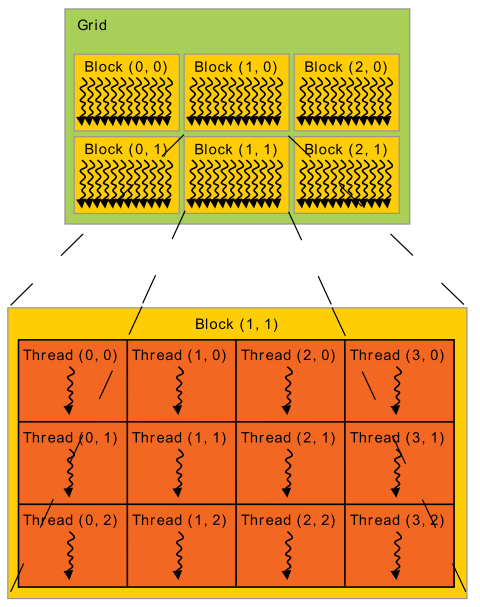
\includegraphics[width=\textwidth]{stateofart/gpgpu/threadgrid}
%         \caption{Thread hierarchy \cite{Nvidia2014}.}
%         \label{fig:gridthread}
%     \end{subfigure}
%     \hfill
%     \begin{subfigure}[b]{0.45\textwidth}
%         \centering
%         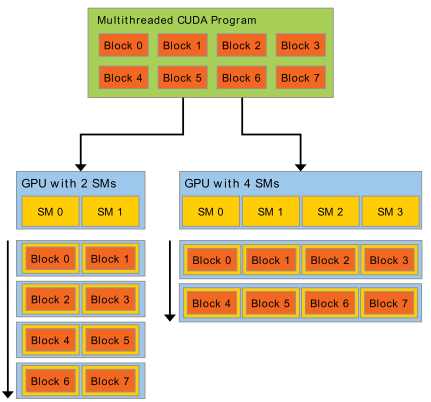
\includegraphics[width=\textwidth]{stateofart/gpgpu/blockprocessor}
%         \caption{Automatic scalability \cite{Nvidia2014}.}
%         \label{fig:blockprocessor}
%     \end{subfigure}
%     \caption{\ref{fig:gridthread} represents the thread hierarchy and \ref{fig:blockprocessor} shows how the distribution of thread blocks is automatically scaled with the increase of the number of multiprocessors.}
%     \label{fig:cuda fig1}
% \end{figure}



Block configuration can be multidimensional, up to and including 3 dimensions.
Furthermore, there is a limit in the amount of threads in each dimension that varies with the GPU being used, e.g. for GPUs with CUDA compute capability 2.x  the maximum number of threads is 1024 for the x- or y-dimensions, 64 for the z-dimension, an overall maximum number of threads of 1024 and a warp size of 32 threads.

Instructions are issued per warp and registers and shared memory are allocated for an active block.
A block will remain active until all threads have finished.
When operands are not ready the warp is stalled and the context switches to another warp.
% This allows for maximizing memory throughput by keeping enough memory transfers running to saturate the memory bus.
Streaming processors have a limit to the maximum number of active warps, depending on the GPU.
Choosing a block size is not trivial, as it is necessary to understand the characteristics of the kernel and the used GPU.
The ratio between the number of active warps per multiprocessor and the maximum number of warps that can be active is called \emph{occupancy} and a high occupancy is often used as a way to choose a good block size.
The idea is to hide latency during global memory loads followed by thread synchronizations by maximizing the number of active warps, i.e. maximizing occupancy.
Occupancy limiters include registers per thread, shared memory per block and threads per block.
% Each streaming processor has a certain amount of registers and if the number of registers per thread times the number of threads per block exceeds the available amount of registers, the launch fails.
NVIDIA supplies a CUDA Occupancy Calculator to aid the programmer in tweaking block size, considering the other limiters.

%For the previous example, it is wise for the number of threads used in a block to be a multiple of 32 to maximize core utilization, otherwise some blocks will have cores that will do no work.

Depending on the architecture, GPUs have several types of memories.
Accessible to all cores (and threads) are the global memory, constant memory and texture memory, of which the last two are read-only.
Blocks share a smaller but significantly faster memory called shared memory, which is a memory inside a multiprocessor to which all cores have access to, enabling inter-thread communication inside a block.
Finally, each thread has access to local memory.
Local memory resides in global memory space and has the same latency for read and write operations.
However, if the thread is using only single variables or constant sized arrays, it uses register space, which is very fast.
If the memory used exceeds the available register space the local memory used.
This memory hierarchy is represented in Figure \ref{fig:memorymodel}.

\begin{figure}[t]
\centering
\begin{minipage}[b]{.5\textwidth}
	\centering
	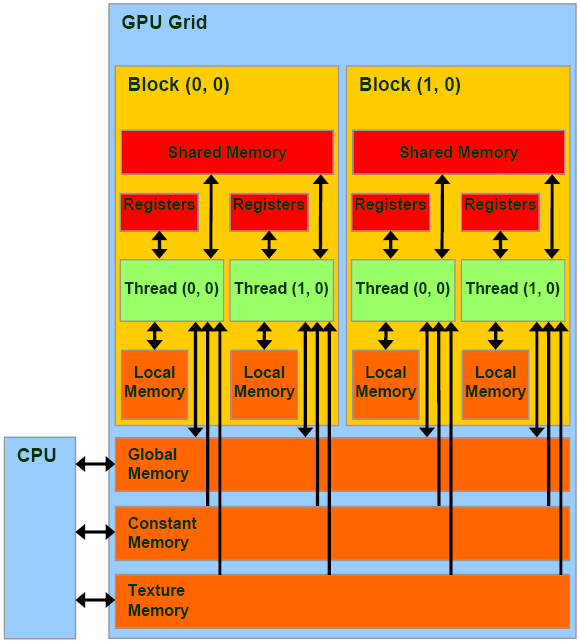
\includegraphics[width=0.9\textwidth]{stateofart/gpgpu/memorymodel}
	\captionof{figure}{Memory model used by CUDA \cite{Nvidia2014}.}
	\label{fig:memorymodel}  
\end{minipage}%
\begin{minipage}[b]{.5\textwidth}
        \centering
        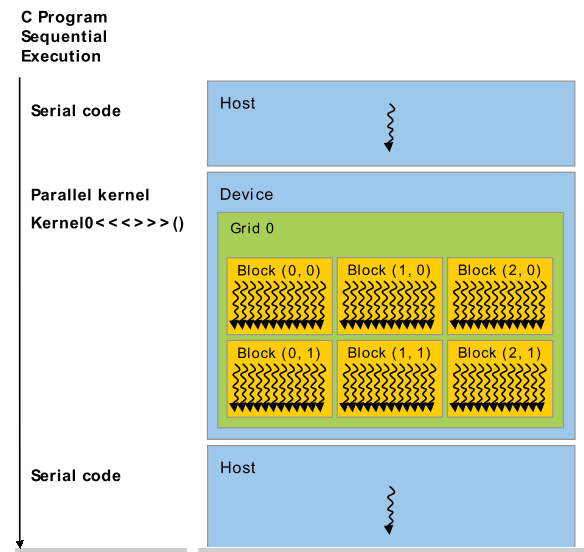
\includegraphics[width=0.9\textwidth]{stateofart/gpgpu/flow}
        \captionof{figure}{Sample execution flow of a CUDA application \cite{Nvidia2014}.}%Automatic scalability 
        \label{fig:cudaflow}
\end{minipage}
\end{figure}

% \begin{figure}[!ht]
%     \centering
%     % this was taken from the internet but is available at NVIDIA slides, could not find a decent reference
%     \begin{subfigure}[b]{0.45\textwidth}
%         \centering
%         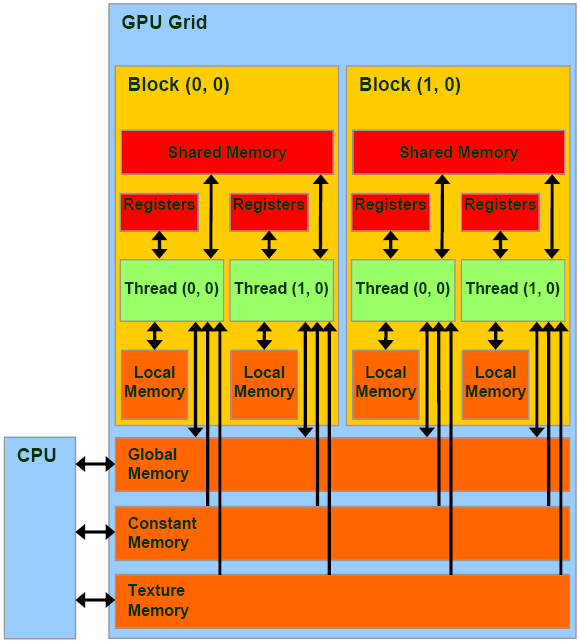
\includegraphics[width=\textwidth]{stateofart/gpgpu/memorymodel}
%         \caption{Memory model used by CUDA \cite{Nvidia2014}.}
%         \label{fig:memorymodel}
%     \end{subfigure}
%     \hfill
%     \begin{subfigure}[b]{0.45\textwidth}
%         \centering
%         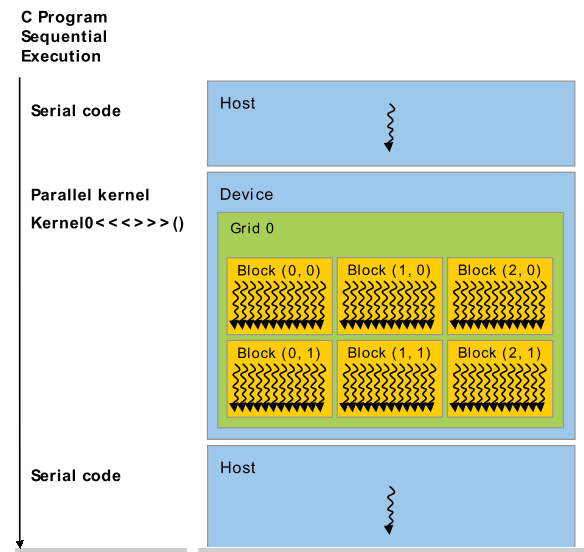
\includegraphics[width=\textwidth]{stateofart/gpgpu/flow}
%         \caption{Sample execution flow of a CUDA application \cite{Nvidia2014}.}
%         \label{fig:cudaflow}
%     \end{subfigure}
%     \caption{}
%     \label{fig:cuda fig2}
% \end{figure}

The typical flow of a CUDA application (and, typically, any modern GPU application) is explained in this paragraph and can be observed in Figure \ref{fig:cudaflow}.
First, the host CPU is responsible for several steps in the set-up phase.
The host starts by transferring any necessary data to the device memory (global, texture or constant).
The next step is selecting the \emph{kernel} (the function that will run on the GPU) and the thread topology (configuration of threads in a block and blocks in the grid).
% First, the host CPU transfers any necessary data to the device memory (global, texture or constant) and is responsible for setting up the device code execution, which entails selecting the \emph{kernel} (the function that will run on the GPU cores) and the thread topology (configuration of threads in a block and blocks in the grid).
The set-up phase is followed by the computation phase in the GPU.
% The next phase is simply the device executing the kernel.
Finally, the host will transfer back the results from the device.
It should be noted that the latest architectures support \emph{Dynamic Parallelism}.
This functionality allows the device to start other kernels without the intervention of the host CPU, which could alter the typical execution flow explained above.
By using this functionality, kernels with data dependencies from other kernels would not require intervention from the host.
Library calls and recursive parallel algorithms are also possible uses.
% Furthermore, additional parallelism is exposed to the GPU's schedulers and load balancers.
% It can be particularly useful if several kernels have data dependencies with other kernels, i.e. their input data is the output from others.
% In such a scenario, a block of the second kernel could be executed as soon as all dependencies were met, effectively cutting overheads for kernel calling from the host CPU.
